\subsection{Configuración de Google Cloud}

Se procede a configurar una cuenta de servicio, mediante la cual se especifican los servicios que se activan desde una instancia generada por una llave en GCP. Esta llave, representada por un archivo JSON, se utiliza para almacenar y recuperar información desde la máquina local. La finalidad de este proceso es la de permitir la interacción con los servicios empleados para el proyecto, posibilitando así la integración con las demás partes del proyecto.

\begin{figure}[h]
	\centering
	\caption{Configuración service account en GCP}
	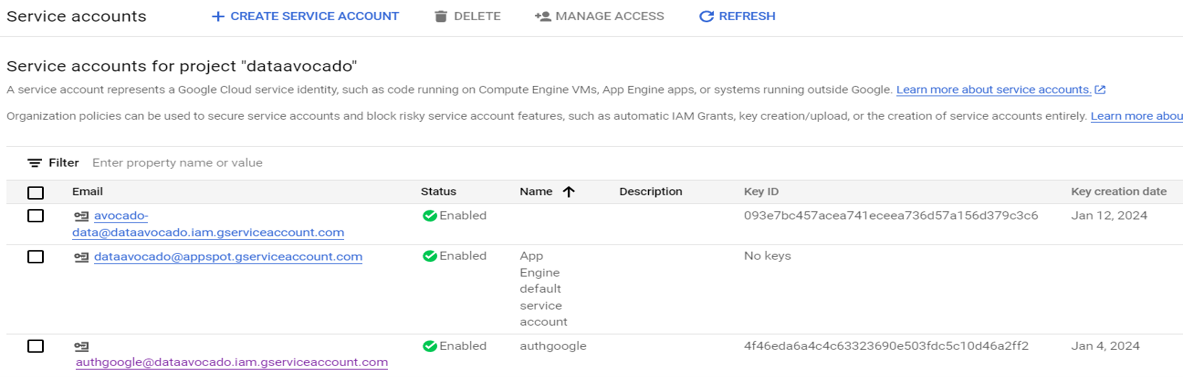
\includegraphics[width=1.1\textwidth]{resultados/configServiceAccount.png}
	\caption*{\footnotesize Fuente: Elaboración propia}
	\label{fig:figuraConfigServiceAccount}
\end{figure}

En el contexto de la configuración de la cuenta de servicio (Service Account), se procede a la creación de una cuenta con el nombre deseado, y posteriormente se configuran los roles permitidos para la manipulación de los servicios de GCP desde dicha cuenta. Por ejemplo, se otorgará a la cuenta, un acceso para el almacenamiento de objetos. Es importante señalar que existen otros roles disponibles que concederían permisos para realizar operaciones como el despliegue de contenedores.

\newpage

\begin{figure}[h]
	\centering
	\caption{Creación del service account en GCP}
	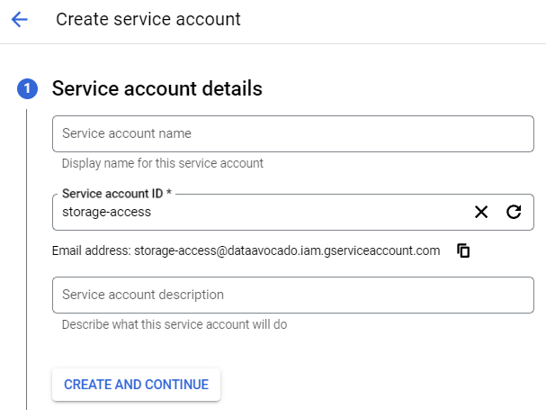
\includegraphics[width=0.6\textwidth]{resultados/creaServiceAccount.png}
	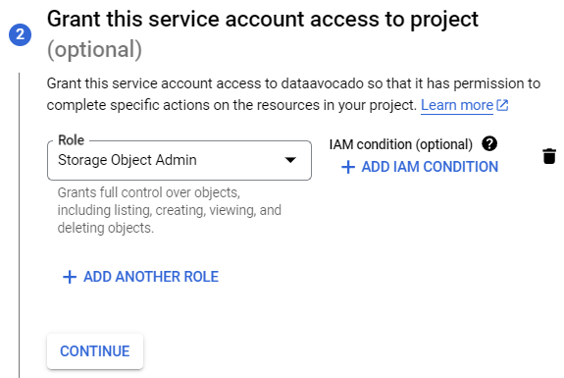
\includegraphics[width=0.6\textwidth]{resultados/creaServiceAccount2.png}
	\caption*{\footnotesize Fuente: Elaboración propia}
	\label{fig:figuraCreaServiceAccount}
\end{figure}

\newpage

\begin{figure}[h]
	\centering
	\caption{Pantallas adicionales del service account en GCP}
	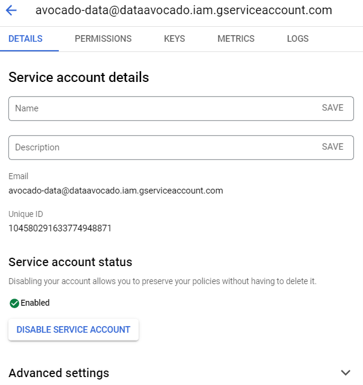
\includegraphics[width=0.5\textwidth]{resultados/adicionalServiceAccount.png}
	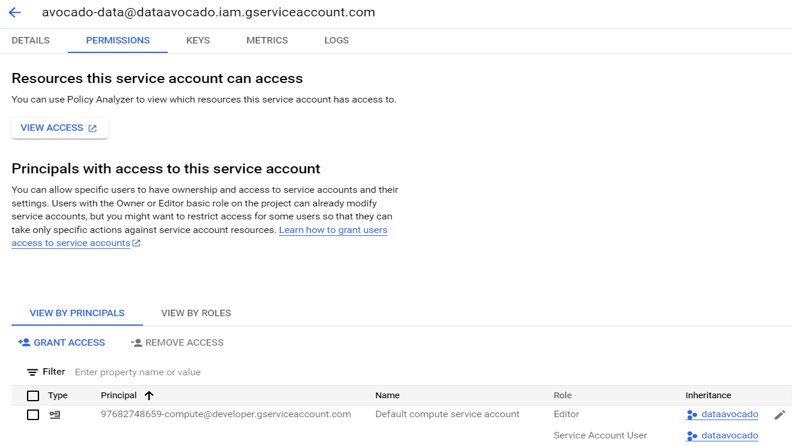
\includegraphics[width=0.6\textwidth]{resultados/adicionalServiceAccount2.png}
	\caption*{\footnotesize Fuente: Elaboración propia}
	\label{fig:figuraAdicionalServiceAccount}
\end{figure}

\newpage

Las figuras anteriores son pantallas adicionales que facilitan la creación de una cuenta de servicio, proporcionando detalles específicos sobre la configuración de dicha cuenta. Para obtener información más detallada acerca de la cuenta de servicio, se puede consultar la documentación de \textbf{Google Cloud Platform} (GCP) \footnote{La documentación referente a cuentas de servicio de GCP se encuentra \href{https://cloud.google.com/iam/docs/service-account-overview?hl=es-419}{aquí}}. \newline

La parte crucial en la creación de la cuenta de servicio implica asignarle un nombre y especificar los roles necesarios para manipular los servicios pertinentes, que en este caso son \textbf{Google Cloud Storage}, \textbf{Google Artifact Registry} y \textbf{Google Cloud Run}. En el proceso, se van añadiendo los roles específicos, como en el caso de haber agregado ``Storage Object Admin''. Se puede continuar agregando los roles necesarios para garantizar que esta cuenta tenga acceso tanto a la gestión de contenedores (Artifact Registry), como a la parte encargada del despliegue de contenedores (Cloud Run) (ver figura \ref{fig:figuraCreaServiceAccount}, figura \ref{fig:figuraAdicionalServiceAccount}). \newline

En la figura \ref{fig:figuraGoogleCloudStorage}, se presenta la interfaz desde \textbf{Google Cloud Storage}, destinada a la creación de un almacenamiento en la nube para los datos. En esta pantalla, se evidencia la existencia de un almacenamiento de datos llamado ``data-project-mlps'', el cual se ha configurado para almacenar toda la información relacionada con los datos que están siendo versionados para el proyecto.

\newpage

\begin{figure}[h]
	\centering
	\caption{Ventana de Google Cloud Storage}
	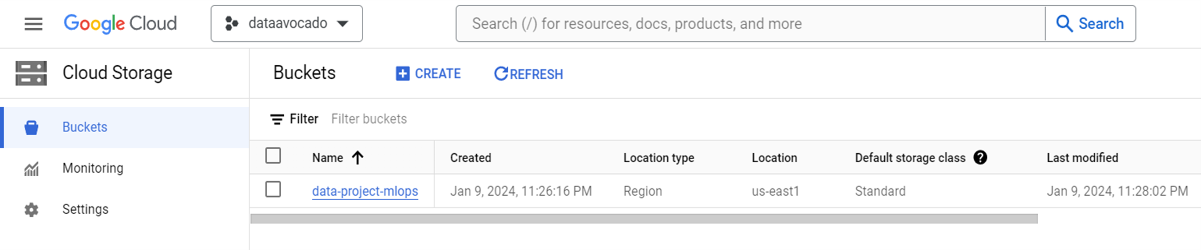
\includegraphics[width=1\textwidth]{resultados/googleCloudStorage.png}
	\caption*{\footnotesize Fuente: Elaboración propia}
	\label{fig:figuraGoogleCloudStorage}
\end{figure}

Al hacer clic en ``data\_project\_mlps'', se accede a una ventana que exhibe información detallada sobre los datos almacenados (ver figura \ref{fig:figuraGoogleCloudStorageDetalle}). Se proporciona el nombre, la ubicación física donde residen los datos y la configuración de acceso público. En este escenario, el acceso público se establece considerando las cuentas de servicio con los permisos necesarios para manipular el almacenamiento de datos en \textbf{Google Cloud Storage}.

\newpage

\begin{figure}[h]
	\centering
	\caption{Ventana de detalle en Google Cloud Storage}
	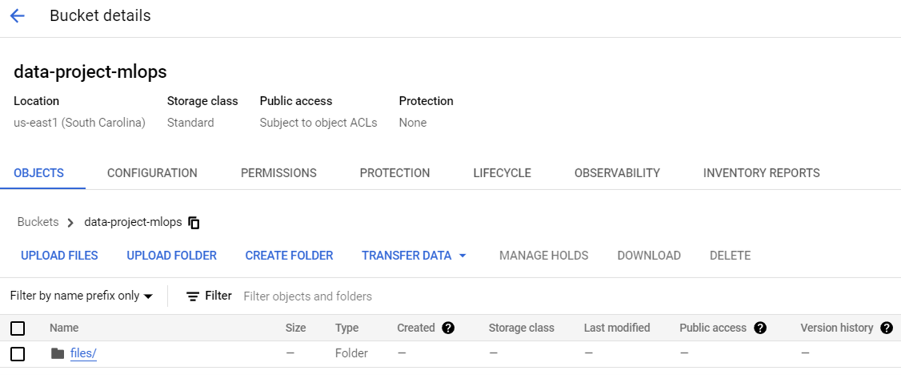
\includegraphics[width=1\textwidth]{resultados/googleCloudStorageDetalle.png}
	\caption*{\footnotesize Fuente: Elaboración propia}
	\label{fig:figuraGoogleCloudStorageDetalle}
\end{figure}

Cuando se opta por la opción ``CREATE’’ (ver figura \ref{fig:figuraGoogleCloudStorage}), se despliega una ventana que permite definir las características del nuevo bucket de almacenamiento (ver figura \ref{fig:figuraGoogleCloudStorageCreacion}). Aquí, se asigna un nombre al bucket que sirve para identificarlo. También se brinda la opción de seleccionar la región de localización, como, por ejemplo, una multi-región para contar con copias de la información en caso de eventos catastróficos o emergencias en una ubicación inicial. Estos puntos de configuración actúan como respaldo, facilitando una recuperación rápida en situaciones adversas en la región predeterminada.

\newpage

\begin{figure}[h]
	\centering
	\caption{Ventana de creación del bucket de almacenamiento en Google Cloud Storage}
	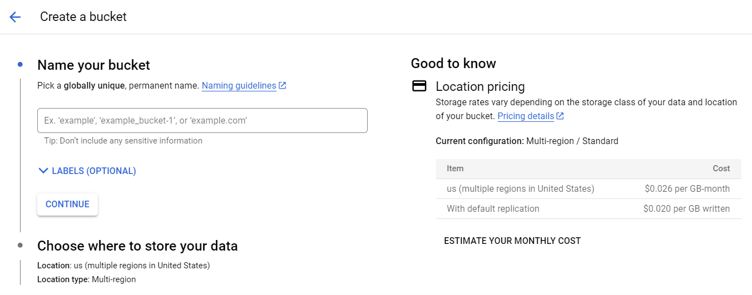
\includegraphics[width=0.7\textwidth]{resultados/googleCloudStorageCreacion.png}
	\caption*{\footnotesize Fuente: Elaboración propia}
	\label{fig:figuraGoogleCloudStorageCreacion}
\end{figure}

\begin{figure}[h]
	\centering
	\caption{Tipo de localización y elección de la clase de almacenamiento en Google Cloud Storage}
	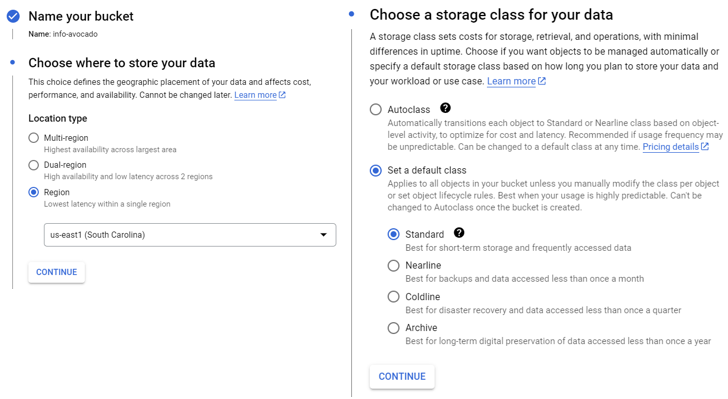
\includegraphics[width=0.8\textwidth]{resultados/googleCloudStorageCreacionDet.png}
	\caption*{\footnotesize Fuente: Elaboración propia}
	\label{fig:figuraGoogleCloudStorageCreacionDet}
\end{figure}

\newpage


No obstante, en el actual proyecto, se ha decidido utilizar únicamente una región, ya que no es un proyecto que, por el momento, tenga una necesidad de escalabilidad masiva. En caso de requerirse, se tiene la flexibilidad de configurar un almacenamiento multi-regional. Sin embargo, es crucial considerar que manejar múltiples regiones o una región dual implica un aumento en los costos, ya que cada región adicional contribuye a un incremento en los gastos asociados. Este aspecto también se refleja en la elección del tipo de almacenamiento necesario para los datos. \newline

Por defecto, se establece el estándar, especialmente cuando se trata de almacenamiento a corto plazo, es decir, datos que pueden cambiar de manera frecuente o no tan frecuente, pero que experimentan modificaciones en ciertos intervalos de tiempo. Aunque existen otras opciones disponibles, la elección de la opción estándar se fundamenta en la necesidad de actualizar datos a medida que la cantidad de información pueda aumentar en el futuro. Esto resulta especialmente relevante cuando un científico de datos planea agregar más datos posteriormente, y la opción estándar proporciona una gestión más eficiente en estas circunstancias. \newline

El control de acceso a este almacenamiento se configura por defecto de manera uniforme, y además, se ofrecen opciones adicionales para proporcionar una capa adicional de protección a los datos, como se describe en la figura \ref{fig:figuraGoogleCloudStorageCreacionControl}. Es importante destacar que, al buscar avanzar o incorporar más características, la complejidad aumenta y, por ende, los costos asociados también. En el proyecto, la elección se ha orientado de esta manera, principalmente por consideraciones educativas y para ajustarse al alcance definido en el proyecto.

\newpage

\begin{figure}[h]
	\centering
	\caption{Elección de control de acceso y protección de datos en Google Cloud Storage}
	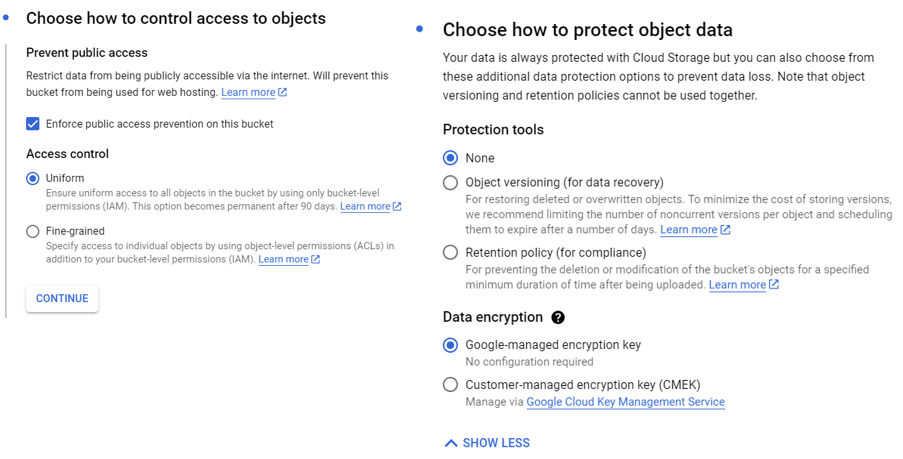
\includegraphics[width=1\textwidth]{resultados/googleCloudStorageCreacionControl.png}
	\caption*{\footnotesize Fuente: Elaboración propia}
	\label{fig:figuraGoogleCloudStorageCreacionControl}
\end{figure}

Adicionalmente, se cuenta con otra herramienta el \textbf{Google Artifact Registry}, destinada específicamente al almacenamiento de contenedores. En esta plataforma, se resguardan tanto el contenedor correspondiente a la API como el asociado a la aplicación (ver figura \ref{fig:figuraGoogleArtifactRegistry}).

\newpage

\begin{figure}[h]
	\centering
	\caption{Ventana de Google Artifact Registry}
	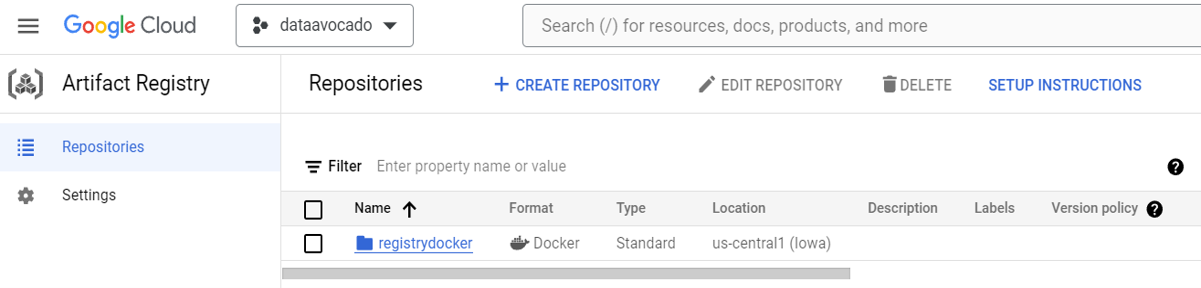
\includegraphics[width=1\textwidth]{resultados/googleArtifactRegistry.png}
	\caption*{\footnotesize Fuente: Elaboración propia}
	\label{fig:figuraGoogleArtifactRegistry}
\end{figure}

Al realizar doble clic en ``registrydocker'', como se visualiza en la figura \ref{fig:figuraGoogleArtifactRegistryDet}, se despliega una ventana que corresponde al repositorio de contenedores creado para el proyecto. En esta interfaz, se presentan los detalles del repositorio, como en donde se encuentran registrados los dos contenedores usados: tanto el de la API como el de la aplicación web. \newline

La interfaz proporcionada por \textbf{Google Cloud Platform} (GCP) permite la creación de un repositorio de contenedores con la capacidad de nombrar los tipos de formatos y modos a guardar (ver figura \ref{fig:figuraGoogleArtifactRegistryCreacion}). Estas opciones se despliegan en las pantallas disponibles en GCP, facilitando la configuración de contenedores según las necesidades específicas de formato y modo.

\newpage

\begin{figure}[h]
	\centering
	\caption{Ventana de detalles del repositorio de contenedores en Google Artifact Registry}
	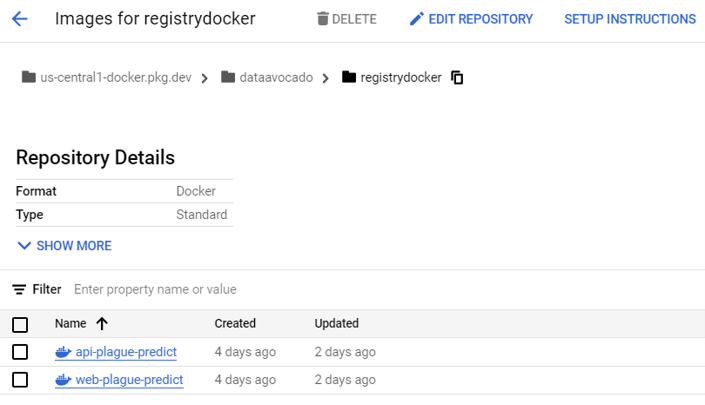
\includegraphics[width=1\textwidth]{resultados/googleArtifactRegistryDet.png}
	\caption*{\footnotesize Fuente: Elaboración propia}
	\label{fig:figuraGoogleArtifactRegistryDet}
\end{figure}

\newpage

\begin{figure}[h]
	\centering
	\caption{Ventana de creación de contenedores en Google Artifact Registry}
	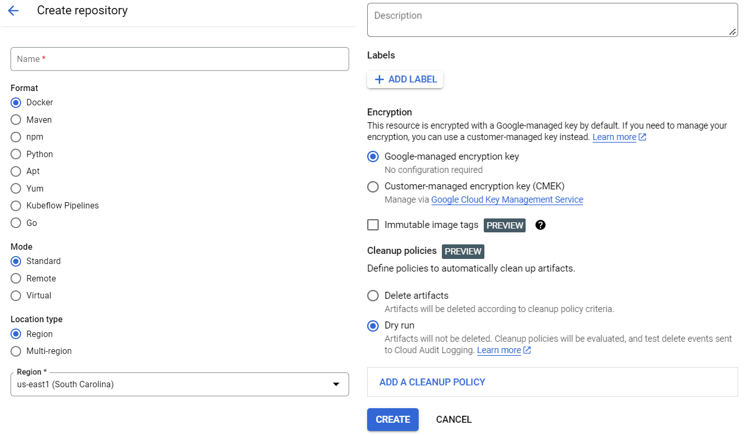
\includegraphics[width=1\textwidth]{resultados/googleArtifactRegistryCreacion.png}
	\caption*{\footnotesize Fuente: Elaboración propia}
	\label{fig:figuraGoogleArtifactRegistryCreacion}
\end{figure}

\newpage

Finalmente, la herramienta \textbf{Google Cloud Run} es la encargada de realizar los despliegues de los contenedores en la nube.

\begin{figure}[h]
	\centering
	\caption{Ventana de Google Cloud Run}
	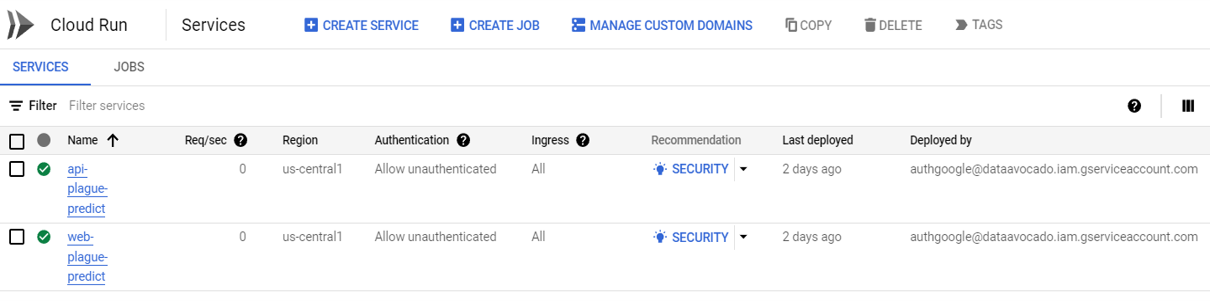
\includegraphics[width=1\textwidth]{resultados/googleCloudRun.png}
	\caption*{\footnotesize Fuente: Elaboración propia}
	\label{fig:figuraGoogleCloudRun}
\end{figure}

Se observa en la figura \ref{fig:figuraGoogleCloudRun}, que ambos contenedores, tanto el de la API como el de la aplicación web, han sido desplegados con éxito. Es importante explicar que, se ha configurado la opción de no permitir la autenticación por defecto, esto se debe a que, de lo contrario, cada vez que se intente acceder a los contenedores, sería necesario proporcionar el usuario y la contraseña de GCP. Dado que se anticipa que otros usuarios utilizarán la API para probar datos y acceder a la aplicación, se ha habilitado la funcionalidad sin necesidad de autorización, permitiendo así un acceso sin restricciones. \newline

En la pestaña del contenedor API (ver figura \ref{fig:figuraGoogleCloudRunDet}), es importante destacar que todo ha sido generado automáticamente por las tareas implementadas en el proyecto con GitHub Actions y no ha sido manipulado manualmente, ya que este es el comportamiento predeterminado. Lo crucial a considerar es que, una vez desplegada la aplicación, se genera una URL (usualmente estática por contenedor) que puede ser accesible por cualquier usuario en internet.

\newpage

\begin{figure}[h]
	\centering
	\caption{Ventana detalle del contenedor API en Google Cloud Run}
	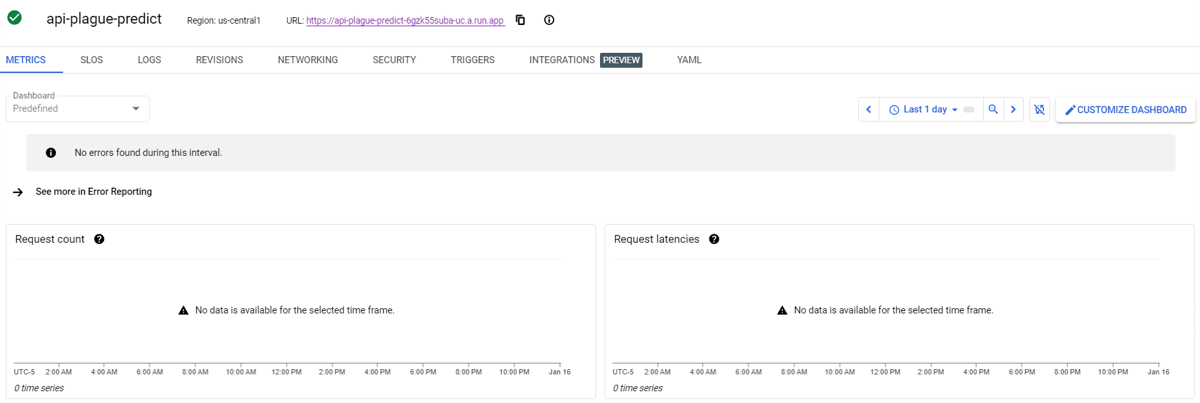
\includegraphics[width=1\textwidth]{resultados/googleCloudRunDet.png}
	\caption*{\footnotesize Fuente: Elaboración propia}
	\label{fig:figuraGoogleCloudRunDet}
\end{figure}

La opción ``CREATE SERVICE'' de la figura \ref{fig:figuraGoogleCloudRun} corresponde a la pestaña destinada a la creación de un servicio (ver figura \ref{fig:figuraGoogleCloudRunCreacion}). Cabe señalar que estos servicios tienen una capacidad limitada, especialmente cuando se utiliza la capa gratuita. Sin embargo, una vez que se excede este límite, se empiezan a generar costos, ya sea por segundos, minutos, horas u diarios, dependiendo de la frecuencia y el uso que se hace de los contenedores.

\newpage

\begin{figure}[h]
	\centering
	\caption{Ventana para crear un servicio en Google Cloud Run}
	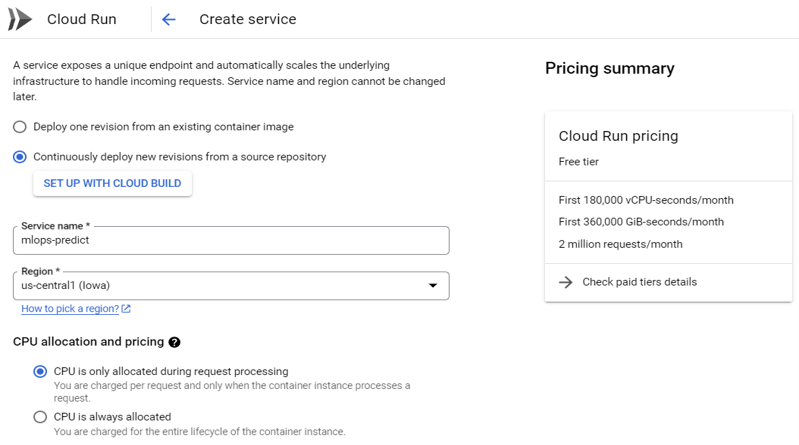
\includegraphics[width=1\textwidth]{resultados/googleCloudRunCreacion.png}
	\caption*{\footnotesize Fuente: Elaboración propia}
	\label{fig:figuraGoogleCloudRunCreacion}
\end{figure}

En cuanto a las opciones de configuración disponibles en \textbf{Google Cloud Run} hay que tener en cuenta lo relacionado con el número máximo de instancias que se desplegarán (ver figura \ref{fig:figuraGoogleCloudRunCreacionDet}). Debido a que esta elección se fundamenta en consideraciones de costos, ya que escalar por ejemplo, desde 3 hasta 100 instancias conllevaría incrementos en los gastos asociados.

\newpage

\begin{figure}[h]
	\centering
	\caption{Ventana de detalles al crear un servicio en Google Cloud Run}
	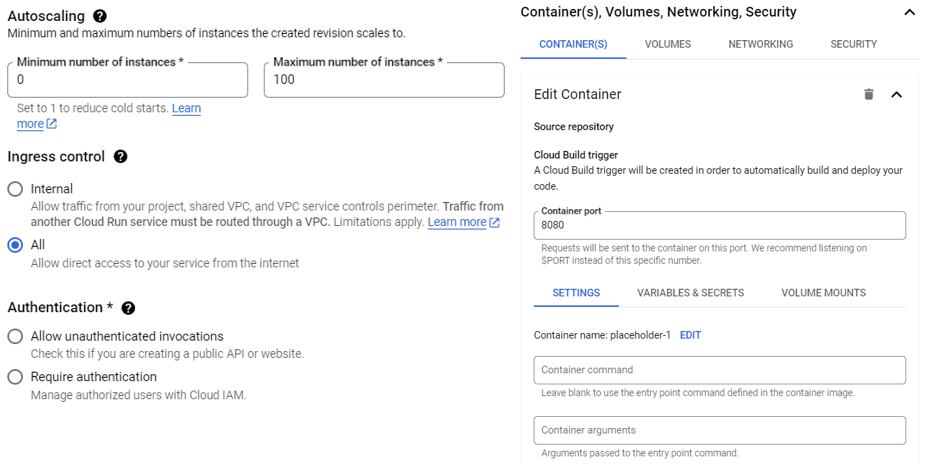
\includegraphics[width=1\textwidth]{resultados/googleCloudRunCreacionDet.png}
	\caption*{\footnotesize Fuente: Elaboración propia}
	\label{fig:figuraGoogleCloudRunCreacionDet}
\end{figure}


Asimismo, especificar en la configuración para permitir una memoria de almacenamiento en 2 GB (ver figura \ref{fig:figuraGoogleCloudRunCreacionRec}) o superior. Esto con el fin de asegurar que el despliegue del proyecto se realice sin problemas de espacio, para los contenedores que se quieran desplegar.

\begin{figure}[h]
	\centering
	\caption{Ventana de detalles al asignar recursos en Google Cloud Run}
	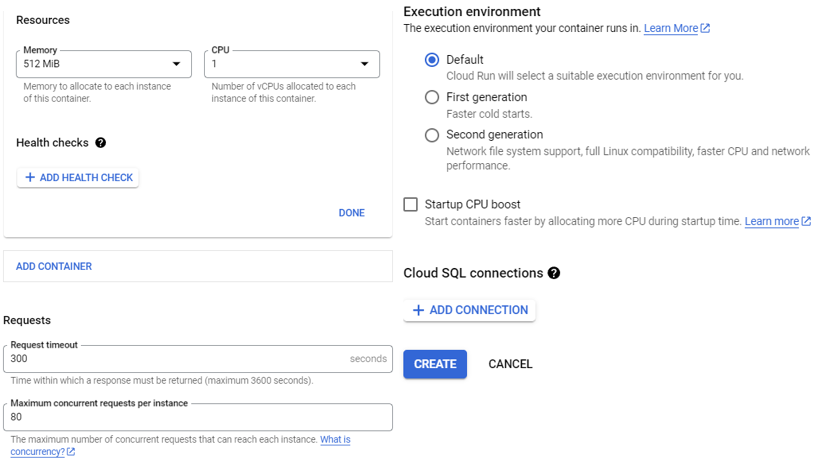
\includegraphics[width=1\textwidth]{resultados/googleCloudRunCreacionRec.png}
	\caption*{\footnotesize Fuente: Elaboración propia}
	\label{fig:figuraGoogleCloudRunCreacionRec}
\end{figure}